\section{Motivation}

Personal, academic, and industrial motivations drive this thesis. It is conducted in collaboration with \textit{Epidemic Sound AB (ES)} \cite{EpidemicSite}, a prominent Swedish company that provides a global library of over 40,000+ royalty-free soundtrack music and 90,000+ sound effects, and the \textit{Music Technology Group (MTG)} at Universitat Pompeu Fabra in Barcelona, Spain. 

The MTG specializes in developing new technologies related to sound and music, including music information retrieval, digital signal processing, computational models of music perception and cognition, and interactive music systems. 

The collaboration with Epidemic Sound and the MTG aims to deepen our understanding of music and its fundamental structures, potentially leading to advancements and benefits for the company's technical products, services, and MIR academic research.

\subsubsection{Personal motivation}

As a music enthusiast, professional musician, and scholar, I am passionately committed to exploring the foundational elements of musical composition, investigating the diverse techniques employed in creating musical works, and deciphering the intricate relationships among them. This passion fuels my quest for knowledge on extracting valuable information embedded within music in any domain, contributing to developing more sophisticated and effective music-related technologies and solutions in the industrial landscape.

I advocate for exposure as the primary method of learning music, emphasizing the importance of immersing oneself in various musical experiences to foster a holistic understanding of music as an art form. Individuals can cultivate well-rounded musical expertise by engaging with different styles, genres, techniques, and learning approaches, ultimately promoting creativity and experimentation in both personal and professional domains.

\subsubsection{Academic motivation}

The emergence of self-supervised models that learn embedding spaces for retrieving musical content from audio signals has unveiled new opportunities in academic research. By capturing high-level semantic information from raw audio data in an unsupervised manner, these models can potentially revolutionize various aspects of the music industry. Their applications encompass music information retrieval, sharing learned latent representations for MIR \cite{HamelTransferSimilarity}, and fostering interdisciplinary research and innovation in musicology, computer science, and artificial intelligence.

\subsubsection{Industrial and corporate motivation}

In the industrial and corporate realm, the embedding spaces generated by these models can be utilized to create personalized and intelligent music recommendation systems \cite{Chen2020LearningRecommendation}\cite{epidemic}, facilitate effective enforcement of intellectual property rights, and contribute to the development of more sophisticated audio editing-production tools and technical products \cite{WonEmotionStories}. These advancements ultimately enhance our interaction with music in the digital age, promoting innovation and collaboration across the music industry.

While it is true that the theoretical foundations of machine learning can be traced back to the pioneering work of figures such as Alan Turing and Claude Shannon in the mid-twentieth century, we are currently experiencing a period of significant breakthroughs in AI research \cite{Vaswani2017AttentionNeed}. These breakthroughs have facilitated the implementation of AI in widely used products \cite{OpenAI2023GPT-4Report}. Many researchers and corporations are keen to stay abreast of these developments and contribute to this exciting and rapidly evolving field.

\subsection{About music aural skills and high-level perceptual concepts}

I have consistently been inspired by musicians and researchers who strive to uncover musical ground truth within an existing tonal paradigm, such as Heinrich Schenker and his school of thought, or by challenging it, exemplified by Arnold Schoenberg or George Russell \cite{LydianRussell}. These approaches aim to identify abstract concepts that reinforce or disrupt the tonal foundation. Their ultimate goal is to advance the tonal landscape, providing musicians with a dependable playground for growth, development, and further understanding of tonal paradigms.

%%%%%%%%%%%%%%%%%%

\begin{figure}[ht]
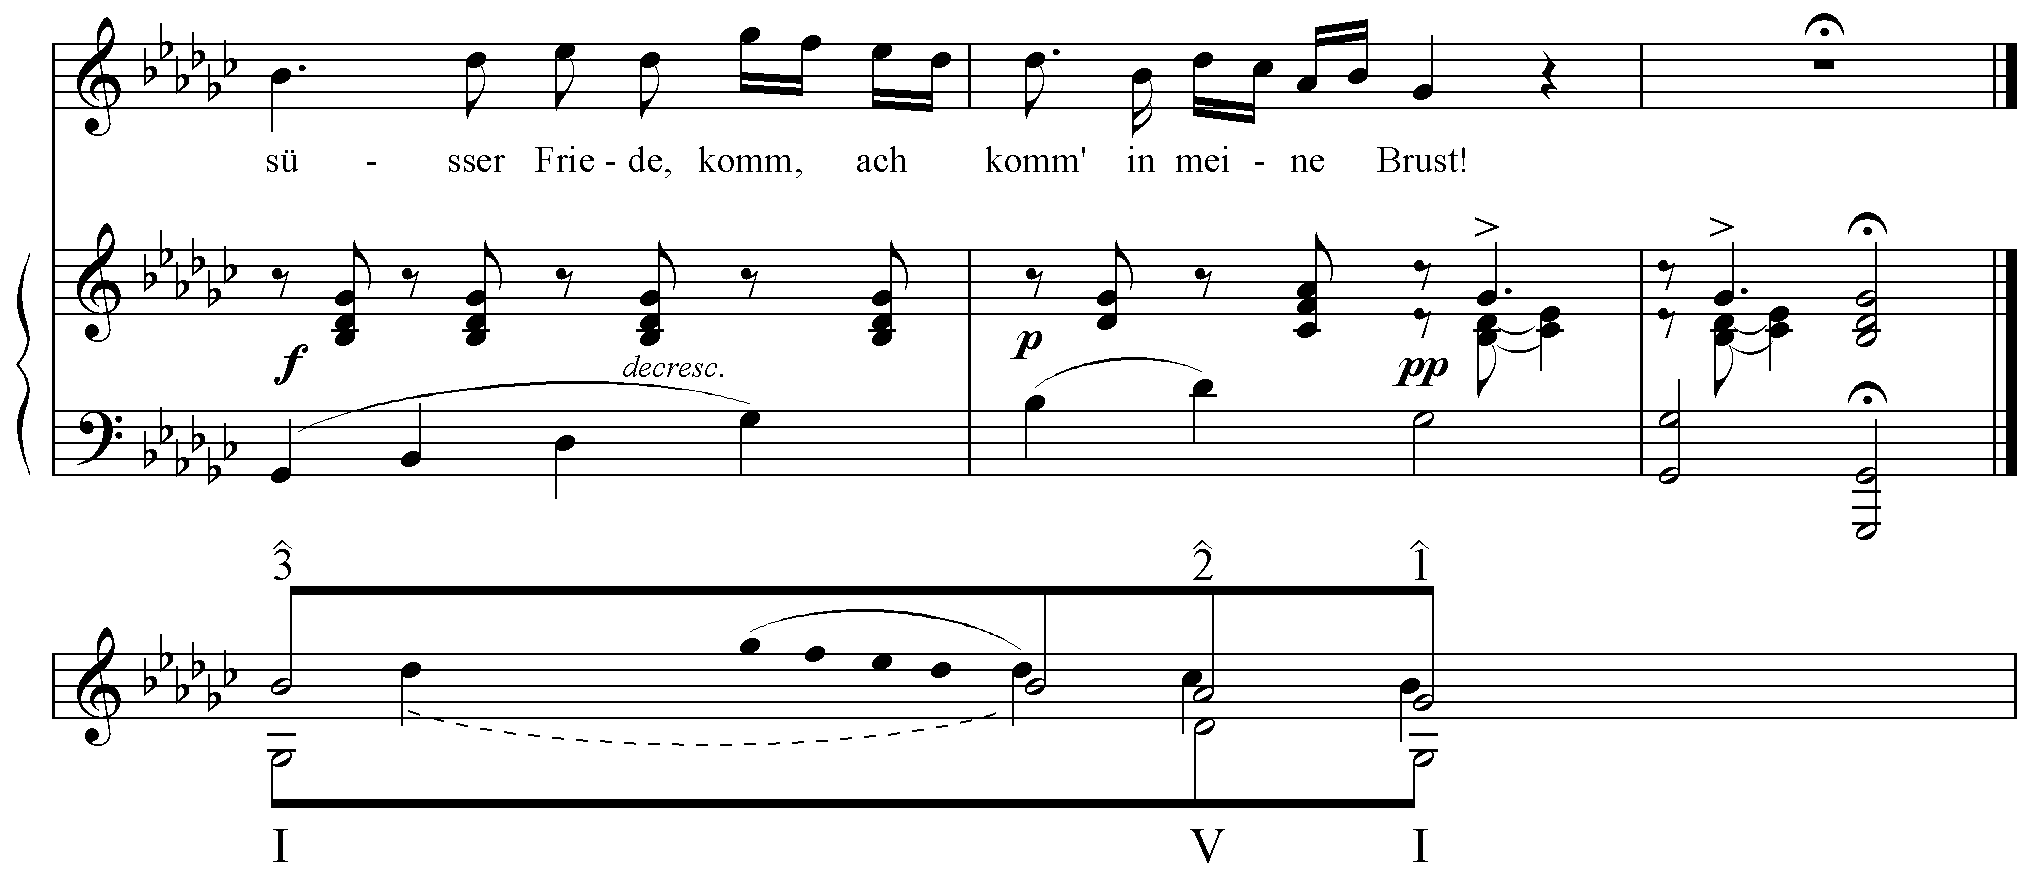
\includegraphics[clip,width=\columnwidth]{figures/schenkerian analysis/SchubertOp4no3.png}% 
\caption{Small excerpt of \textit{Wandrers Nachtlied, Op. 4, D. 224} by Franz Schubert. We can see the passage's original score, the schenkerian unfolding of the melody, the chord degrees analysis, and the tonal function.}
\label{fig:Wandrers Nachtlied, Op. 4, D. 224}
\end{figure}

%%%%%%%%%%%%%%%%%%%%%%%%%%%%%%%%%%%%%%%%%%%%

Schenkerian Analysis, developed by Austrian music theorist Heinrich Schenker, investigates the underlying structure of tonal music by focusing on the hierarchical relationships between pitches. This analytical approach is founded on the premise that all tonal music shares a fundamental structure known as "Ursatz" or "basic shape." The method identifies a piece's stepwise descending line (Urlinie) and bass arpeggiation (Bassbrechung), simplifying it to its essential elements and examining how different layers contribute to the overall structure. Central concepts in Schenkerian Analysis include prolongation levels, harmony, counterpoint, voice-leading, and Ursatz (fundamental structure). Despite criticism for reducing all tonal works to a limited number of background structures, Schenker highlights the significance of individual elaboration in determining a piece's identity and meaning.

While such analysis is designed for the symbolic domain, we argue that musical abstraction is also feasible in the audio time domain. In this section, we explore the application of Schenkerian Analysis principles to the Music Information Retrieval (MIR) domain by examining the foreground, middle-ground, and background levels of musical structure as follows:

\begin{itemize}
\item \textbf{Foreground}: The surface level of a musical composition, consisting of the notes, rhythms, and articulations directly perceived by the listener, representing the most detailed level of the musical structure.

\item \textbf{Middle-ground and mesostructures}: An intermediate level of analysis focusing on essential structural elements such as harmonic progressions, thematic materials, and voice-leading reductions that contribute to the overall composition. In the MIR domain, this level can also be understood as mesostructure. Mesostructures are intermediate levels of articulation between waveshapes' microstructure and musical forms' macrostructure. Examples of mesostructures include melody, arpeggios, syncopation, polyphonic grouping, and textural contrast. Mesostructures might have received limited attention in deep learning, as current models only focus on microstructures \cite{Mesostructures2023}.

\item \textbf{Background}: The most abstract level of musical structure, representing the fundamental core consisting of the \textit{Urlinie} and \textit{Bassbrechung}, which serves as the foundation for the entire composition.
\end{itemize}

By understanding and applying Schenkerian Analysis principles to the MIR domain, we can better understand the complex relationships between different levels of musical structure in the audio time domain, allowing for a more comprehensive analysis of tonal music.

\subsection{Beyond Digital Signal Processing (DSP)}

We argue that MIR research needs to incorporate a more balanced approach that considers the interdisciplinary nature of music and the importance of other domains beyond DSP.

\subsubsection{Sample MIR task}

Let's pick a core MIR task as a sample to display such complexity: Music Structure Analysis (MSA), an interdisciplinary field that aims to understand the structure of music \cite{Nieto2020Audio-BasedApplications}. However, due to subjectivity, ambiguity, and data scarcity, audio-based MSA faces challenges like boundary placement ambiguity and similarity quantification \cite{NietoPerceptualMusic}. 

The main principles of MSA were initially defined as homogeneity, novelty, and repetition, with the addition of regularity. The checkerboard kernel technique is a simple and effective method for MSA based on the homogeneity principle. The kernel, with a checkerboard-like structure, is convolved over the main diagonal of a Self-Similarity Matrix (SSM) such as $S_{ij}$ is the similarity between time frames $i$ and $j$, $\vec{x}_i$ is the vector representation of time frame $i$, and $\left| \vec{x}_i \right|$ is the Euclidean norm of vector $\vec{x}_i$. The dot product of two vectors $\vec{x}_i$ and $\vec{x}_j$ is denoted by $\vec{x}_i \cdot \vec{x}_j$.

\begin{equation}
\label{eq:segment_similarity}
S_{ij} = \frac{\vec{x}_i \cdot \vec{x}_j}{\left\| \vec{x}_i \right\| \left\| \vec{x}_j \right\|}
\end{equation}

This yields a novelty curve highlighting sudden changes in the selected musical features from which to extract the segment boundaries.

\begin{equation}
n_i = \frac{\sum\limits_{j=1}^{N} S_{ij} - N\cdot S_{ii}}{\sqrt{\sum\limits_{j=1}^{N} (S_{ij} - S_{ii})^2}}
\end{equation}

Where $N$ is the number of time frames, $S_{ij}$ is the similarity between time frames $i$ and $j$, $S_{ii}$ is the similarity between time frame $i$ and itself, and $n_i$ is the novelty value for time frame $i$.

The numerator of the expression represents the sum of similarities between time frame $i$ and all other time frames minus the average similarity across all time frames. The denominator of the expression is the standard deviation of the similarities, which is used to normalize the values to ensure that the novelty values are between -1 and 1.


Mathematical operations are used on predefined principles such as homogeneity and repetition to analyze a musical structure. It explores features extracted from a musical signal and identifies peaks in a novelty curve to extract segment boundaries. In contrast, human aural skills rely on the perception and interpretation of music by human listeners based on cultural and academic background. They can capture subtle nuances of musical structure, but those still are subjective and can vary across listeners.

Combining technical tasks, aural skills, and music perception is challenging due to the complexity and subjectivity of musical perception, discrepancies between the features extracted by DSP techniques and the features perceived by humans, and the variability of musical signals and individual differences in musical perception. 

Purely mathematical approaches may not always reflect how humans perceive music and may not capture the subtle variations in timing or harmonic relationships critical to musical perception. Variability in musical signals due to instrumentation, genre, and performance style further complicates the development of these techniques that can be generalized to different musical contexts.